\chapter{幂指对函数}
\begin{introduction}
    \item 幂函数
    \item 指数函数
    \item 对数函数
    \item 双钩函数
\end{introduction}

\section{幂函数}
\subsection{幂函数的定义}
\begin{definition}[幂函数]
    形如$f(x)=x^k$（其中$k\in \mathbb{Q}$为常数）的函数称为幂函数。
\end{definition}
\begin{note}[幂运算]
    从小学到初中我们依次学会了\\
    正整数幂：
    $$
        x^2 = x\times x
    $$
    负整数幂：
    $$
        x^{-n} = \frac{1}{x^n}
    $$
    分数幂：
    $$
        x^{\frac{1}{n}} = \sqrt[n]{x}
    $$
    于是我们可以算出所有的有理数幂：
    $$
        x^{\frac{p}{q}} = \sqrt[q]{x^p}
    $$
\end{note}
\subsection{幂函数的图像}
幂函数的性质取决于$k$的取值。

$k=0$时为常函数：
\begin{figure}[H]
    \centering
    \begin{tikzpicture}
        \draw[<->](3,0)--(0,0)--(0,3);
        \draw(0,-2)--(0,0)--(-3,0);
        \draw[blue,domain=-1.8:1.8] plot(\x,1);
    \end{tikzpicture}
    \caption{$y=1$}
\end{figure}
$k$为正整数时：
\begin{figure}[H]
    \centering
    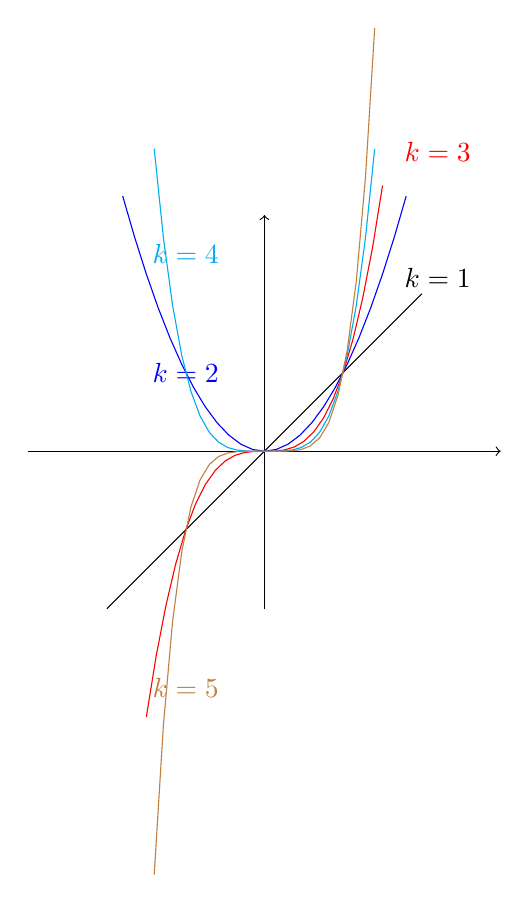
\begin{tikzpicture}
        \draw[<->](3,0)--(0,0)--(0,3);
        \draw(0,-2)--(0,0)--(-3,0);
        \draw[black,domain=-2:2] plot(\x,\x) node at (2.2,2.2) {$k=1$};
        \draw[blue,domain=-1.8:1.8] plot(\x,\x*\x) node at (-1,1) {$k=2$};
        \draw[red,domain=-1.5:1.5] plot(\x,\x^3) node at (2.2,3.8) {$k=3$};
        \draw[cyan,domain=-1.4:1.4] plot(\x,\x*\x*\x*\x) node at (-1,2.5) {$k=4$};
        \draw[brown,domain=-1.4:1.4] plot(\x,\x*\x*\x*\x*\x) node at (-1,-3) {$k=5$};
    \end{tikzpicture}
    \caption{正整数}
\end{figure}
$k$为负整数：
\begin{figure}[H]
    \centering
    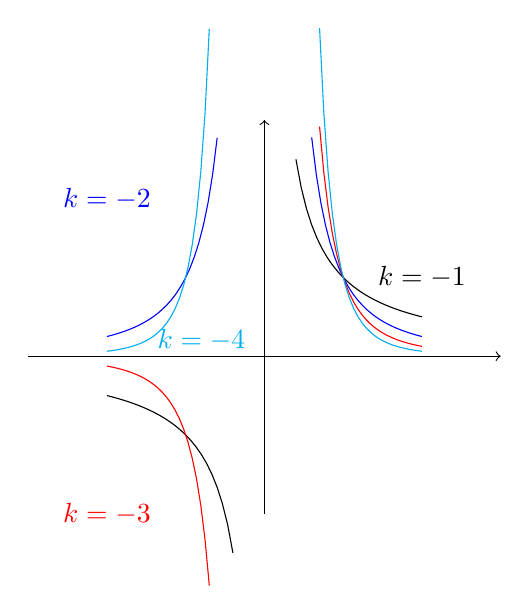
\begin{tikzpicture}
        \draw[<->](3,0)--(0,0)--(0,3);
        \draw(0,-2)--(0,0)--(-3,0);
        \draw[black,domain=-2:-0.4] plot(\x,1/\x) node at (2,1) {$k=-1$};
        \draw[black,domain=0.4:2] plot(\x,1/\x);
        \draw[blue,domain=-2:-0.6] plot(\x,{1/(\x)^2}) node at (-2,2) {$k=-2$};
        \draw[blue,domain=0.6:2] plot(\x,{1/(\x)^2});
        \draw[red,domain=-2:-0.7] plot(\x,{1/(\x)^3}) node at (-2,-2) {$k=-3$};
        \draw[red,domain=0.7:2] plot(\x,{1/(\x)^3});
        \draw[cyan,domain=-2:-0.7] plot(\x,{1/(\x)^4}) node at (-0.8,0.2) {$k=-4$};
        \draw[cyan,domain=0.7:2] plot(\x,{1/(\x)^4});
    \end{tikzpicture}
    \caption{负整数}
\end{figure}
$k$为分数：
\begin{figure}[H]
    \centering
    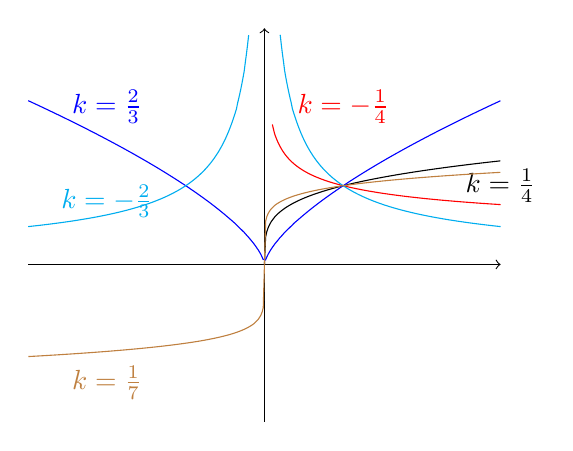
\begin{tikzpicture}
        \draw[<->](3,0)--(0,0)--(0,3);
        \draw(0,-2)--(0,0)--(-3,0);
        \draw[black,domain=0:3,samples=200] plot(\x,{\x^0.25}) node at (3,1) {$k=\frac{1}{4}$};
        \draw[red,domain=0.1:3,samples=200] plot(\x,{\x^(-0.25)}) node at (1,2) {$k=-\frac{1}{4}$};
        \draw[blue,domain=-3:3,samples=200] plot(\x,{((\x)^2)^(1/3))}) node at (-2,2) {$k=\frac{2}{3}$};
        \draw[cyan,domain=-3:-0.2,samples=200] plot(\x,{1/(((\x)^2)^(1/3)))}) node at (-2,0.8) {$k=-\frac{2}{3}$};
        \draw[cyan,domain=0.2:3,samples=200] plot(\x,{1/(((\x)^2)^(1/3)))});
        \draw[brown,domain=0:3,samples=200] plot(\x,{(\x)^(1/7)}) node at (-2,-1.5) {$k=\frac{1}{7}$};
        \draw[brown,domain=0:3,samples=200] plot(-\x,{-(\x)^(1/7)});
    \end{tikzpicture}
    \caption{分数}
\end{figure}
分数的情况较为复杂，如果分母是偶数那么根据分数幂的定义，自变量不能取负值。
\section{指数函数}
\subsection{指数函数的定义}
\begin{definition}[指数函数]
    形如$f(x)=a^x$（其中$a>0$为常数）的函数称为指数函数。
\end{definition}
\subsection{指数函数的图像}
指数函数的图像较为简单，不考虑$a=1$这种非平凡情况。

当$a>1$时，函数单调增：
\begin{figure}[H]
    \centering
    \begin{tikzpicture}
        \draw[<->](3,0)--(0,0)--(0,4);
        \draw(0,-1)--(0,0)--(-3,0);
        \draw[black,domain=-2:1] plot(\x,{2^(\x)}) node at (1.6,2) {$a=2$};
        \draw[blue,domain=-2:1] plot(\x,{3^(\x)}) node at (1.6,3) {$a=3$};
        \draw[red,domain=-2:1] plot(\x,{4^(\x)}) node at (1.6,4) {$a=4$};
    \end{tikzpicture}
    \caption{$a>1$}
\end{figure}
当$a<1$时，函数单调增：
\begin{figure}[H]
    \centering
    \begin{tikzpicture}
        \draw[<->](3,0)--(0,0)--(0,4);
        \draw(0,-1)--(0,0)--(-3,0);
        \draw[black,domain=-1:2] plot(\x,{(1/2)^(\x)}) node at (-1.5,2) {$a=\frac{1}{2}$};
        \draw[blue,domain=-1:2] plot(\x,{(1/3)^(\x)}) node at (-1.5,3) {$a=\frac{1}{3}$};
        \draw[red,domain=-1:2] plot(\x,{(1/4)^(\x)}) node at (-1.5,4) {$a=\frac{1}{4}$};
    \end{tikzpicture}
    \caption{$a<1$}
\end{figure}
\section{对数函数}
\subsection{对数函数的定义}
\begin{definition}[对数函数]
    形如$y=\log_ax$（其中$a\in (0,1)\cup (1,\infty)$）的函数称为对数函数。
\end{definition}
\begin{note}[对数]
    在数学的应用中我们常常需要解决这样的问题：
    $$
        2^x=3
    $$
    也就是回答这样一个问题：$2$的多少次方是$3$。

    这个问题的答案不是一个简单的有理数，而是一个无理数。为了方便表达，我们把这个数记作$\log_23$，读作以2为底3的对数。其中的$\log$是英语Logarithm的前三个字母。

    我们常用的对数有
    \begin{enumerate}
        \item 以2为底的$\log_2x$
        \item 以10为底的$\log_{10}x$，也写作$\lg x$
        \item 以$e$为底的$\log_ex$，也写作$\ln x$，称为自然对数。其中$e\approx 2.71828$，称作自然对数的底数。和$\pi$一样是一个无理数。
    \end{enumerate}
\end{note}
\begin{definition}[自然对数的底数]
    $e$和$\pi$类似，是数学中最重要的常数之一。

    圆周率$\pi$的定义大家都知道，“周三径一”，也就是：
    $$
        \pi = \frac{\text{周长}}{\text{直径}}
    $$

    这里也给出一个$e$的定义：
    $$
        e = \frac{1}{0!}+\frac{1}{1!}+\frac{1}{2!}+\frac{1}{3!}+\frac{1}{4!}+\cdots
    $$
    其中$n!=n\times(n-1)\times(n-2)\times\cdots\times 2\times 1$称为阶乘。读者可以用计算器验证$e\approx 2.71828$。
\end{definition}
\subsection{对数的性质}
\begin{enumerate}
    \item 吸收乘数$$n\log_ab = \log_ab^n$$
    \item 分裂$$\log_a(xy) = \log_ax+\log_ay$$
    \item 负数$$-\log_ax = \log_{1/a}x$$
    \item 换底公式$$\log_ab = \frac{\log_cb}{\log_ca}$$
\end{enumerate}
利用幂运算的性质可以比较容易地证明以上性质。
\begin{exercise}[无理数证明]
    证明：$\log_23$是无理数。
\end{exercise}
\begin{proof}
    假设$\log_23$是有理数，那么
    $$
        \exists m,n \in \mathbb{N} \quad \log_23=\frac{m}{n}
    $$
    也就是
    $$
        n\log_23=m
    $$
    根据对数的性质可以得到
    $$
        \log_23^n = \log_22^m
    $$
    于是
    $$
        3^n=2^m
    $$
    这个等式左侧是奇数，右侧是偶数，显然矛盾。所以假设不成立，也即$\log_23$是无理数。
\end{proof}
\subsection{对数函数的图像}
对数函数的图像也比较简单。

当$a>1$时，函数单调增：
\begin{figure}[H]
    \centering
    \begin{tikzpicture}
        \draw[<->](4,0)--(0,0)--(0,4);
        \draw(0,-3)--(0,0)--(-1,0);
        \draw[black,domain=0.3:4] plot(\x,{log10(\x)/log10(2)}) node at (4.8,2) {$a=2$};
        \draw[blue,domain=0.3:4] plot(\x,{log10(\x)/log10(3)}) node at (4.8,1.3) {$a=3$};
        \draw[red,domain=0.3:4] plot(\x,{log10(\x)/log10(4)}) node at (4.8,1) {$a=4$};
    \end{tikzpicture}
    \caption{$a>1$}
\end{figure}

当$a<1$时，函数单调减：
\begin{figure}[H]
    \centering
    \begin{tikzpicture}
        \draw[<->](4,0)--(0,0)--(0,4);
        \draw(0,-3)--(0,0)--(-1,0);
        \draw[black,domain=0.3:4] plot(\x,{-log10(\x)/log10(2)}) node at (4.8,-2) {$a=1/2$};
        \draw[blue,domain=0.3:4] plot(\x,{-log10(\x)/log10(3)}) node at (4.8,-1.3) {$a=1/3$};
        \draw[red,domain=0.3:4] plot(\x,{-log10(\x)/log10(4)}) node at (4.8,-1) {$a=1/4$};
    \end{tikzpicture}
    \caption{$a<1$}
\end{figure}

\subsection{指数函数和对数函数}
不难发现指数函数和对数函数是存在反函数对应关系的。

例如$y=e^x$和$y=\ln x$互为反函数，他们的图像关于直线$y=x$对称。

\section{双钩函数}
这里我们特别介绍一个函数：
$$
    y=x+\frac{1}{x}
$$
它的图像为：
\begin{figure}[H]
    \centering
    \begin{tikzpicture}
        \draw[<->](4,0)--(0,0)--(0,4);
        \draw(0,-4)--(0,0)--(-3,0);
        \draw[blue,domain=0.3:3] plot(\x,{\x+1/\x});
        \draw[blue,domain=-3:-0.3] plot(\x,{\x+1/\x});
        \draw[dotted] (-3,-3)--(3,3);
    \end{tikzpicture}
    \caption{$y=x+1/x$}
\end{figure}
酷似两个对勾，因此俗称双钩函数。

根据基本不等式，在第一象限
$$
    y=x+\frac{1}{x}\geq 2
$$
当且仅当$x=1$的时候取等号。

并且$y=x+\frac{1}{x}$中，$1/x$随着$x$的增大快速减小，最终由$x$主导整个函数的取值，所以不难想象该函数图像会越来越向$y=x$靠近，这种行为我们称为渐进，$y=x$称为$y=x+\frac{1}{x}$的\textbf{渐近线}。

\begin{problemset}
    \item 解方程：$3^x+4^x+5^x = 6^x$
\end{problemset}